\subsection{Interrelación Asignatura - Asignatura Curso Académico}

   \begin{description}
      \item[Definición] En esta interrelación se deja constancia de que una
      asignatura se desarrolla durante un determinado curso académico.

      \item[Características] La interrelación presenta las siguientes
                             características:

         \begin{itemize}
            \item \textbf{Nombre:} A-ACA
            \item \textbf{Tipo de la interrelación:} El tipo de entidad
                  Asignatura Curso Académico es débil por identificación
                  respecto al tipo de entidad Asignatura.
            \item \textbf{Cardinalidad de la interrelación:} 1:N
            \item \textbf{Número de atributos:} Ninguno.
         \end{itemize}

      \item[Diagrama] La figura \ref{diagramaA-ACA} muestra el diagrama de la
                      interrelación.

      \item \begin{figure}[!ht]
            \begin{center}
            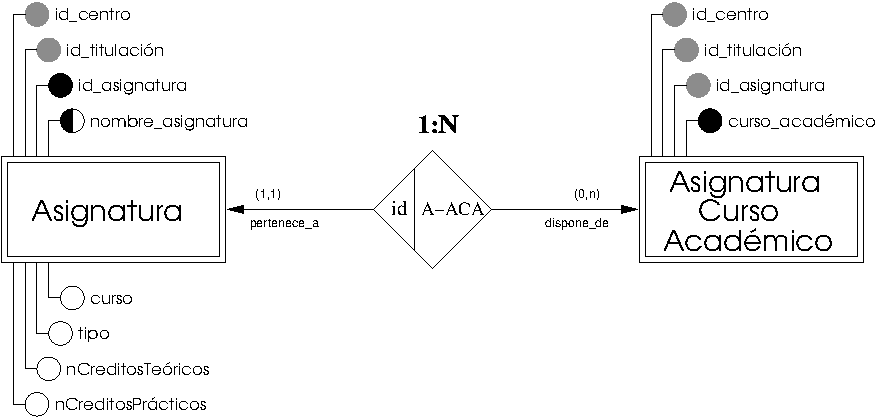
\includegraphics[]{07.Modelo_Entidad-Interrelacion/7.3.Analisis_Interrelaciones/diagramas/A-ACA.pdf}
            \caption{Diagrama de la interrelación A-ACA.}
            \label{diagramaA-ACA}
            \end{center}
         \end{figure}

      \item[Ejemplo práctico del tipo de interrelación]

      \item \begin{center}
            \begin{tabular}{ | c | c | }
            \hline
            \multicolumn{2}{ | c | }{\textbf{Tipo de interrelación A-ACA}} \\
            \hline
            \textbf{Asignatura} & \textbf{Asignatura Curso Académico}\\
            \hline
            id\_centro+id\_titulación+id\_asignatura & id\_centro+id\_titulación+id\_asignatura+curso\_académico \\
            \hline
            15317 & 153172008 \\
            \hline
            \end{tabular}
         \end{center}
   \end{description}
